\documentclass{article}
\usepackage{geometry}
\usepackage[document]{ragged2e}
\usepackage{csquotes}
\usepackage{hyperref}
\usepackage{graphicx}
\geometry{a4paper,total={170mm,257mm},left=20mm,top=20mm}
\newcommand\independent{\protect\mathpalette{\protect\independenT}{\perp}}
\def\independenT#1#2{\mathrel{\rlap{$#1#2$}\mkern2mu{#1#2}}}
\begin{document}
    \begin{titlepage}
        \begin{center}
            \vspace*{1cm}
            
            \textbf{Probabilistic Models Project Proposal}
            
            \vspace{0.5cm}
            
            
            \vspace{1.5cm}
            
            \vfill
            
            Final Project\\
            
            \vspace{0.8cm}
            
            
            
            Computer Science\\
            IDC\\
            \today
            
        \end{center}
    \end{titlepage}
    \textbf{Intro}\\
    Probabilistic Graphical Models (PGM) use a graph representation to describe complex distribution over high dimensional space. Where Every node in the graph correspond a random variable, and edges in the graph correspond to direct probabilistic interactions between variables. This representation is a set of in-dependencies holds in the distribution.\\
    In high dimensional distribution the graph representation encode the probability in small factors rather then over every possible assignment of the variables, and the joined distribution defined as the a product of all these factors. In this kind of representation we can define Bayesian network and Markov network distributions in a visual way. Where the Bayesian network is represented as a directed graph and Markov as undirected graph.\\
    This representation allow humans to better evaluate properties and semantics of a variables distribution, it can help understand unexplained or undesirable answers. In addition using the graph to analyses data, it is possible to run efficient algorithm to posterior probability of variables given the evidence of others. Another characteristic is learning from data model provides a good approximation of past experience.\\~\\

    The main objective of this project is to develop a user-friendly software tool for constructing PGMs and experimenting with different aspects and inference algorithms. This tool will be designed both for educational use in academic courses and for self exploration by scientists and developers in the industry. This tool illustrates different aspects of probabilistic models in 6 different units:
    \begin{enumerate}
        \item Unit 1 - conditional independence in Bayesian networks\\
                Learn basic concepts in probabilistic models. Visual independence using Bayesian network, including D separation
        \item Unit 2 - undirected representations of Bayesian networks\\
                Objective is to see a different representation of Bayesian network
        \item Unit 3 - elimination orders\\
                Learn how to calculate joint probability for some nodes in Bayesian network, and marginal probability for some set of variables in the network
        \item Unit 4 - inference algorithms
        \item Unit 5 - parameter inference
        \item Unit 6 - sampling algorithms on general Probabilistic Graphical Models
    \end{enumerate}
    A more comprehensive explanation on every unit can be found in proposed design section. The tool designed to experiment basic understanding from dependencies of random variables, until running different algorithms on Bayesian networks.\\~\\

    In our research we came across a couple of libraries implements different algorithms on PGMs. Although those libraries have some aspects in common with our tool, we believe our tool helps to experiment in PGMs more gradually. Most of the libraries offer an efficient code, sometimes with visual representation, but not for learning purposes. Here is the list of tools:
    \begin{enumerate}
        \item Kevin Murphy - THe most comprehensive tool we found, an assemble of Matlab libraries implements various probabilistic models. Most of the libraries written by Kevin Murphy along with his students. Some of the libraries are:
            \begin{enumerate}
                \item PMTK - A collection of Matlab functions, written to support Kevin Murphy textbook ``Machine learning: a probabilistic perspective''.
                \item DAG structure learning using L1 regularization - A library to find Markov blankets using L1
                \item Bayesian DAG learning - Bayesian inference over DAG (directed acyclic graph). This library cannot handle undirected graphs and inference with hidden nodes.
            \end{enumerate}
        \item Hidden Markov Model Toolbox - Written By Kevin Murphy in 1998, support inference for HMMs (Hidden Markov Model), implemented on Matlab
        \item OpenGM - A C++ Implementation for discrete factor graph models. The main objective of this library is to give efficient implementation, and not a learning experience.
        \item Probabilistic Graphical Models - A Matlab implementation for inference and learning Bayesian and Markov networks hosted on Github. The library gives a code to learn PGM, but lack the visualization part.
    \end{enumerate}

    \pagebreak

    \textbf{Implementation Demo}
    \begin{figure}[h!]
        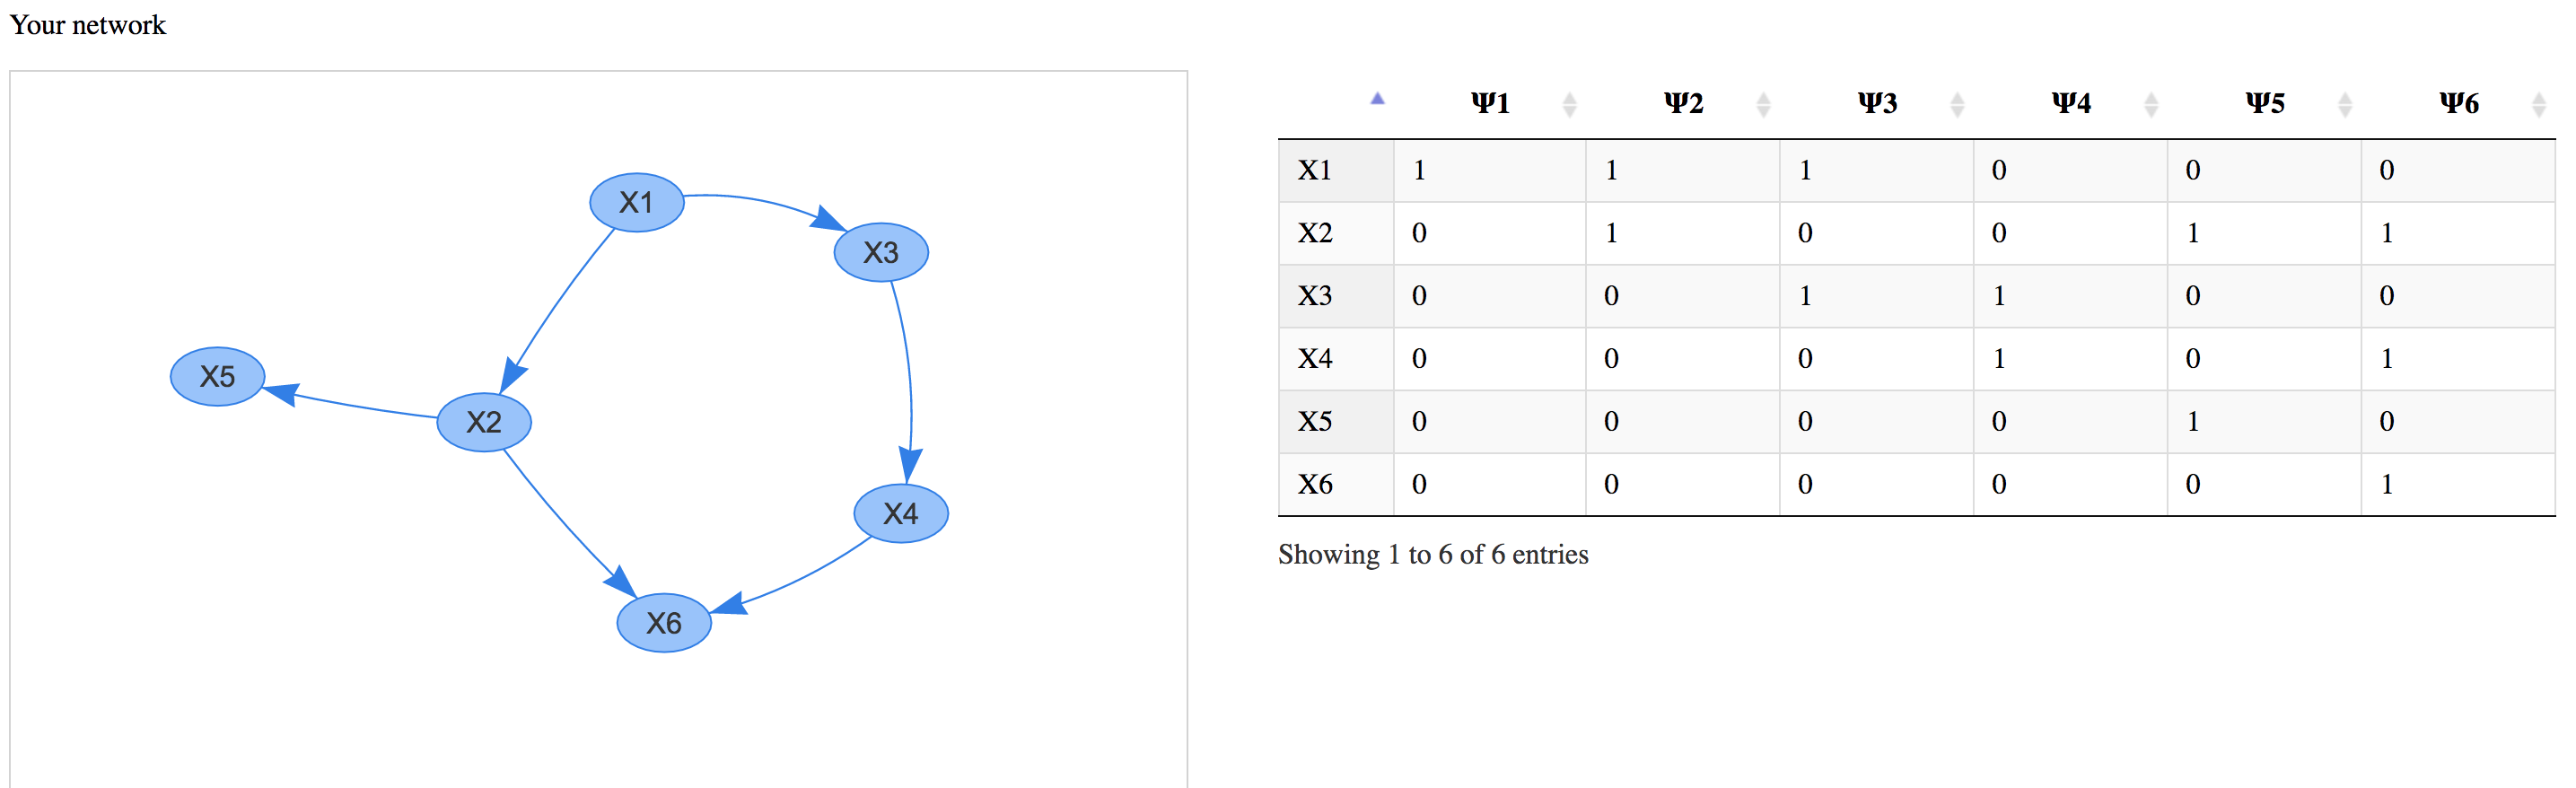
\includegraphics[width=\linewidth]{img/network_binary_matrix.png}
        \caption{Bayesian network representation by DAG with binary matrix.}
        \label{fig:besian_network}
    \end{figure}

    \begin{figure}[h!]
        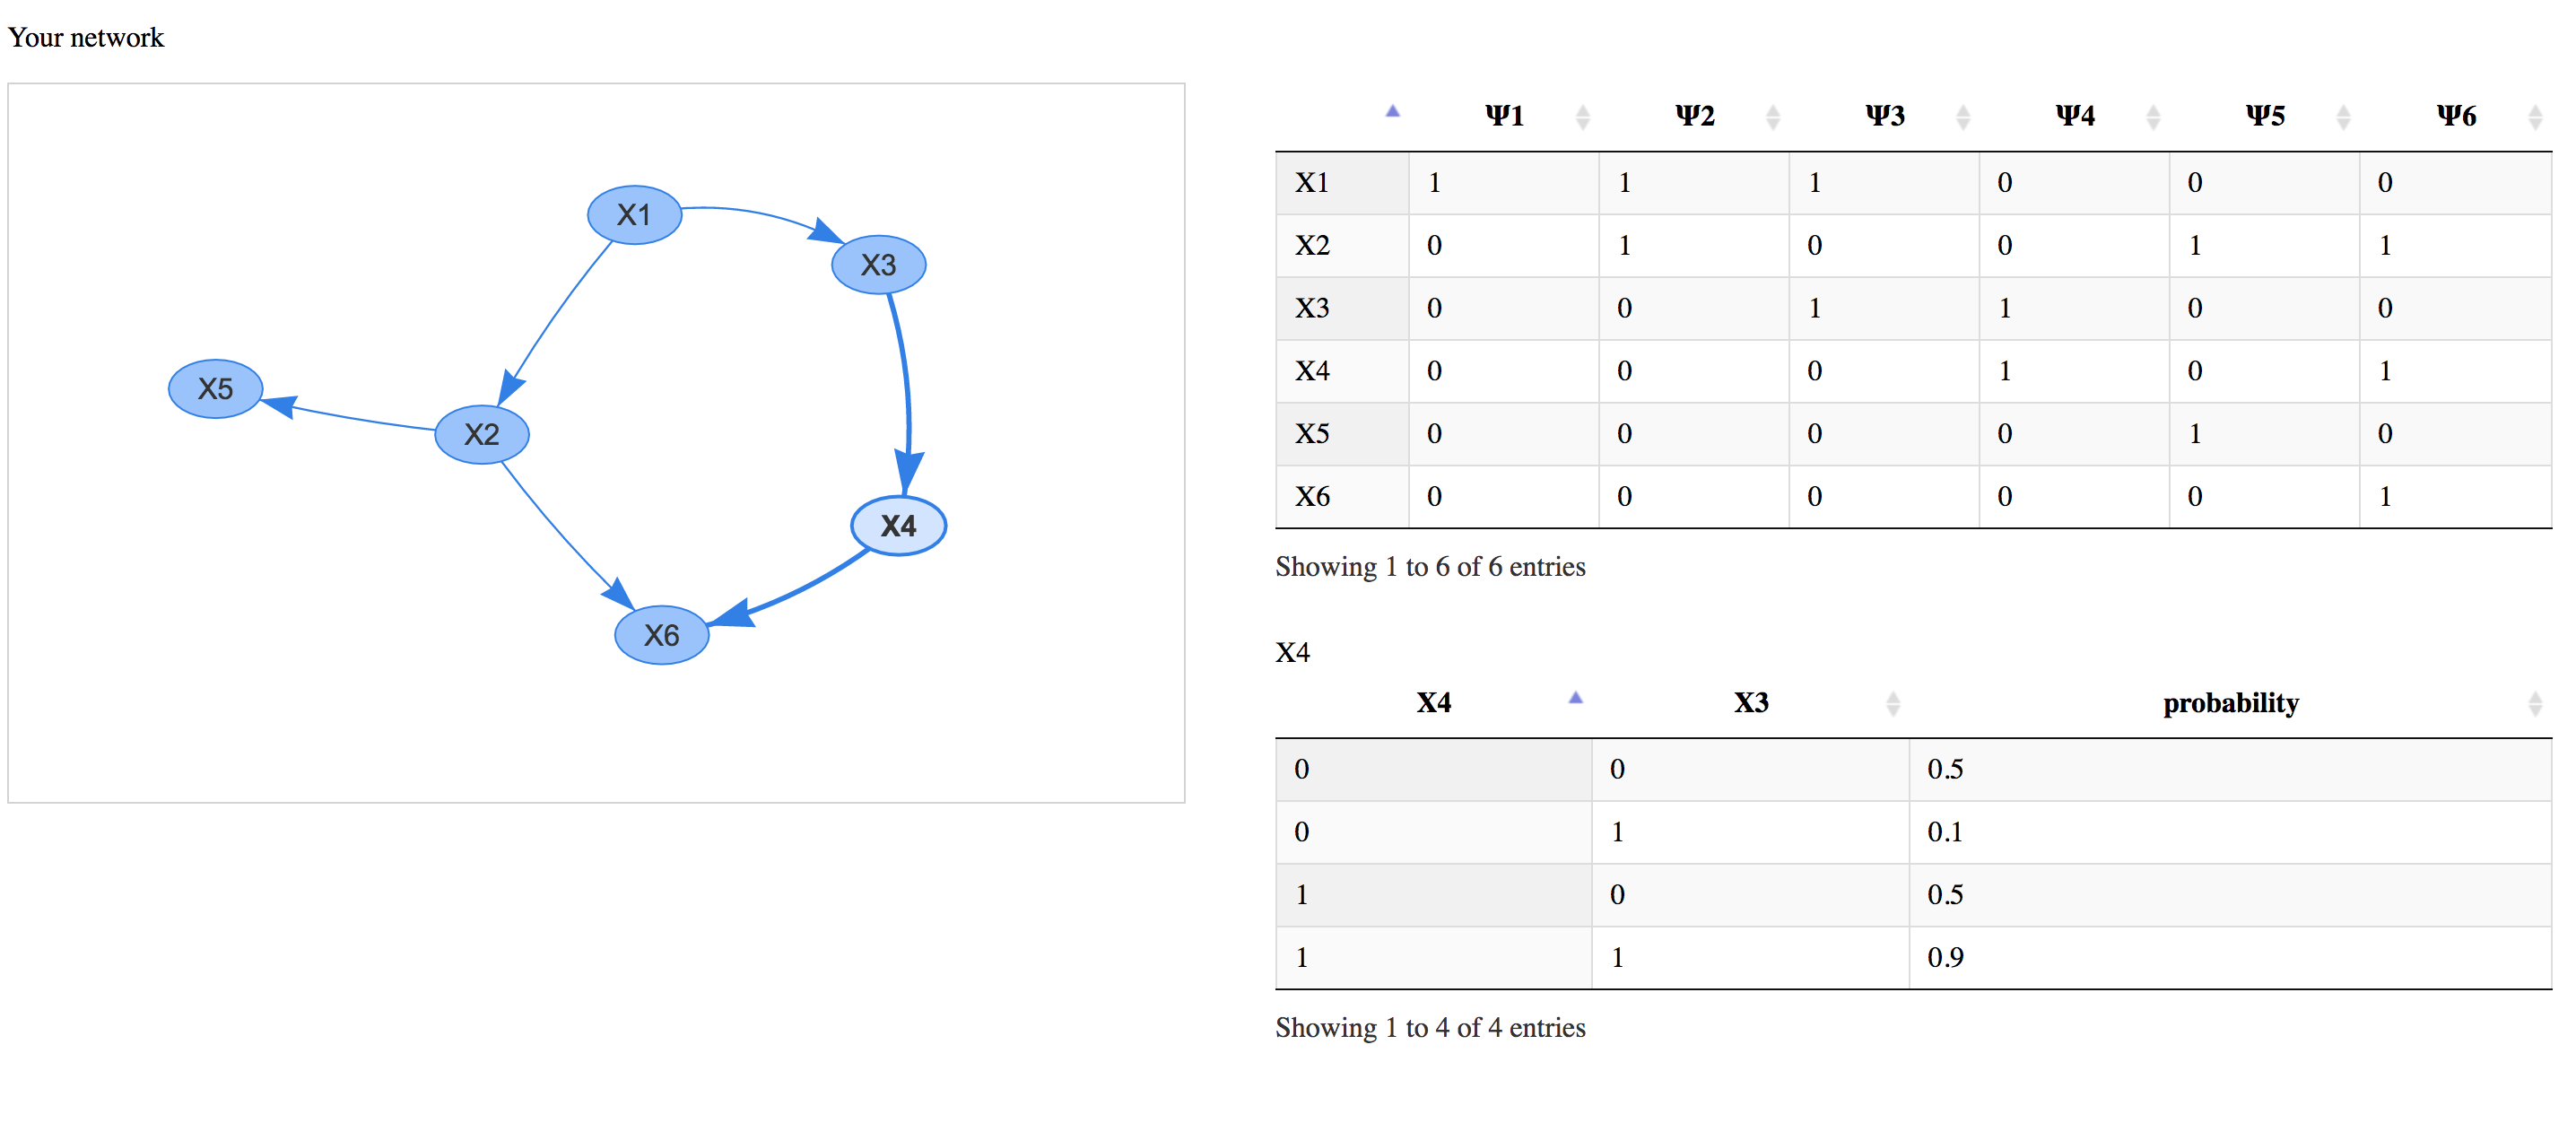
\includegraphics[width=\linewidth]{img/network_selected_node_table.png}
        \caption{Bayesian network representation by DAG, after one node is chosen, show it's potential function table.}
        \label{fig:besian_network_chosen_node}
    \end{figure}
    \vspace{0.5cm}

    \textbf{Proposed Design}\\
    As stated in the introduction the tool is build from 6 units, in this section we are going to elaborate on each one. Every unit extends the capabilities of the former unit.
    \begin{enumerate}
        \item Unit 1\\
        This unit is the designed to learn the basics of probability modeling of data. After understanding the basics in probability, visualize
        dependency in discrete random variables using a Bayesian network.
        \begin{enumerate}
            \item Use predefined Bayesian networks to illustrate dependence vs independence in random variables
            \item Allow the user to define a Bayesian network, and define dependency between variables. The graph representation is giving the user the ability to better understand the network.
            \item show conditional independence using D separation rules. The D separation is a general criterion for deciding from a given graph whether a set of variables X are independent of another set U given another set A. Or more formally: $X_V \independent X_U | X_A$.\\The rules are:\\
            \begin{enumerate}
                \item Path contains a node $w \in A$ and not both adages that touch w are incoming:
                \begin{enumerate}
                    \item $X_u \rightarrow x \rightarrow X_v$
                    \item $X_u \leftarrow x \leftarrow X_v$
                    \item $X_u \leftarrow x \rightarrow X_v$
                \end{enumerate}
                \item path contains a node $w\notin A$ with two incoming edges $X_u \rightarrow w \leftarrow X_v$
            \end{enumerate}
            The user is going to be able to choose two nodes, the tool is going to show id those nodes are depended or not using D separation. If they are conditional
            independent show the user all the paths that does not block dependency, otherwise show the path that block dependency.\\
        \end{enumerate}

        \vspace{0.5cm}

        \item Unit 2\\
        This unit objective is understanding the undirected graph representation of the Bayesian network.
        \begin{enumerate}
            \item 
             Covert graph representation of a model to moralized graph. This is an undirected representation every two variables in the same conditional table have an edge. Create an undirected version of the Bayesian network, where two RVs v u have an edge iff  $P(X_u | X_v) or P(X_v | X_u) or P(X_z | X_v, X_u) $. Emphasize that nodes associated with a potential function form a clique in the graph.\\
            \item Validate if graph is chordal or not. The main characteristic of this graph is that every cycle of four or more vertices have a chord, in other words every included cycle in the graph should have exactly three vertices. 
            \item Convert moralized graph to factor graph. A bipartite graph representation with one class representing nodes in original graph and the other class representing maximal cliques. As stated in this representation it is easier to see the maximal cliques in the graph.
        \end{enumerate}
        \item Unit 3\\
            The main objective of this unit is to see inference 
        \begin{enumerate}
            \item Show elimination algorithm implementation on graphs.
            \begin{enumerate}
                \item Show elimination in moralized graph. The user can choose an elimination order, the moralized graph will reflect how the elimination of a node creates new edges for the node neighbors (if needed).
            \end{enumerate}
            \item Find perfect elimination for tree. The perfect elimination can be found using the moralized graph from unit 2, validate if the graph is chordal or not.
            \item Show message passing algorithm in graph representation. Display the marginal distribution tables of vertexes along the algorithm.
        \end{enumerate}
        \item Unit 4\\
        \begin{enumerate}
            \item Parameter inference through data in tree models
        \end{enumerate}
        \item Unit 5\\
        \begin{enumerate}
            \item Markov chain Monte Carlo algorithm
        \end{enumerate}
    \end{enumerate}

    \textbf{Model Representation}\\
    A model is represented using:
    \vspace{0.1cm}
    \begin{enumerate}
        \item Random variables. Where every random variable can have:
        \begin{enumerate}
            \item Name (X)
            \item Domain $\Omega$ where every x in $\Omega$ have the probability $P(X=x)$
        \end{enumerate}
    \end{enumerate}
    Example for JSON file, representation of random variable\\
    variable:\\
            \-\quad - name: x1\\
            \-\quad\quad   domain:\\
            \-\quad\quad - 0\\
            \-\quad\quad - 1\\
            \-\quad - name: x2\\
            \-\quad\quad   domain:\\
            \-\quad\quad - 0\\
            \-\quad\quad - 1\\
            \-\quad\quad - 2\\
    
    \textbf{Visual Representation}\\
    \begin{enumerate}
        \item Represent Bayesian network using DAG. Represent all the nodes, with the direct edges from parents to node $P(X_v | X_{\pi_v})$
        \item Represent the elimination algorithm for a Bayesian network. $f(x_{hidden})=P(x_{hidden},X_{observed})=\sum_{\forall x \in V}P(X_v|X_{\pi_v})$. This is designed to show the elimination algorithm step by step.\\
        Setup:\\
        \begin{enumerate}
            \item Set all the nodes data and with the observed nodes value.
            \item set the elimination order
        \end{enumerate}
        Initialization:\\
        \begin{enumerate}
            \item Set potential function for all the nodes $\Psi_{v \in V}$, where $\psi_v = P(X_v|X_{\pi_v})$
            \item create a matrix $|V\setminus observed| X |\Psi|$ of all RVs associate with every potential function.
            \item Set the list of elimination order of RVs in $X_{V\setminus (observed \cup infered)}$
        \end{enumerate}
        Elimination Loop:\\
        \begin{enumerate}
            \item $X_v$ is the next RV in the elimination order so $\Psi_v$ is the potential functions have RV in the matrix
            \item $n(X_v)$ are the RVs that involved in one of the potential function in $\Psi_v$
            \item set $m_v$ of all RVs in $n(X_v)$. So $m_v(n(X_v))=\sum_{X_v}\Psi_v$
            \item replace $\Psi_v$ with $m_v$
        \end{enumerate}
        By setting up elimination order the user is able see the impact on the complexity.\\
        Output of the run - the elimination step by step with potential matrix.

        \item Convert Bayesian network to moralized graph. In this scenario the objective is to show how the operation is done step by step.

        \item Message passing algorithm. Visual representation of the message passing. Step by step running of eliminate procedure

        \item Factor Tree and message passing algorithm. Represent the conversion between a direct graph to the moralized version and then to factor graph
    \end{enumerate}

    \vspace{0.1cm}
    \textbf{CLI tool}\\
    \begin{enumerate}
        \item Running elimination algorithm for given node setup with elimination order.\\
        Command: eliminate \enquote{path to file} \enquote{elimination order for all the nodes}\\
        Input:\\
        \begin{enumerate}
            \item JSON file path, representing the RVs, nodes and conditional tables for all nodes $P(X_v=x_v|X_{\pi_v}=x_{\pi_v})$.
            \item elimination order of the nodes
        \end{enumerate}
        Output:\\
        Joint probability $f(\overline{x_{infered}})=P(X_{infered},X_{observed})$\\

        

        \item Message passing algorithm in trees. Run only eliminate procedure.
        Command: message passing \enquote{sync/async} \enquote{path to file} \enquote{elimination order for all the nodes}\\
        Give the ability to run in two modes:\\
        \begin{enumerate}
            \item synchronous - eliminate one child of a node at a time
            \item asynchronous - eliminate child nodes in parallel
        \end{enumerate}
        Message passing algorithm with compute marginal for all nodes. Run the procedures collect and distribute\\

        \item Message passing with most probable joint assignment. The input is the same as the other message passing CLI arguments. The output in this case is maximum probability and the assignment.

        \item Run message algorithm on poly tree. Given as input:\\
        Command: message passing \enquote{sync/async} \enquote{path to file} \enquote{elimination order for all the nodes}\\
        \begin{enumerate}
            \item poly tree with nodes V and edges E
            \item conditional tables for all nodes $P(X_v=x_v|X_{\pi_v}=x_{\pi_v})$
        \end{enumerate}
        Output:\\
        Marginal distribution for all the nodes
    \end{enumerate}

    \vspace{0.5cm}
    \begin{thebibliography}{9}
        \bibitem{Kevin Murphy}
        Kevin Murphy and students libraries \\\texttt{http://www.cs.ubc.ca/\~{}murphyk/Software/}
        \bibitem{Hidden Markov Model Toolbox}
        Kevin Murphy toolbox for inference on Hidden Markov Models \\\texttt{http://www.cs.ubc.ca/\~{}murphyk/Software/HMM/hmm.html}
        \bibitem{OpenGM}
        OpenGM C++ library for discrete graph models \\\texttt{http://hciweb2.iwr.uni-heidelberg.de/opengm/}
        \bibitem{Probabilistic Graphical Model Library} 
        A code implementation of different aspects in PGMs
        \\\texttt{https://github.com/anhncs/Probabilistic-Graphical-Models}
    \end{thebibliography}
\end{document}